% !TeX root = ../../tesi.tex

For RGB acquisition at Site~2, the \textbf{Raspberry Pi Camera Module~3 Wide} was employed.\cite{raspberrypi_camera_module_3_2026} This device is an official Raspberry Pi imaging sensor designed for embedded vision applications and directly interfaced to the Raspberry Pi 5 through the CSI camera interface.

\begin{figure}[h]
    \centering
    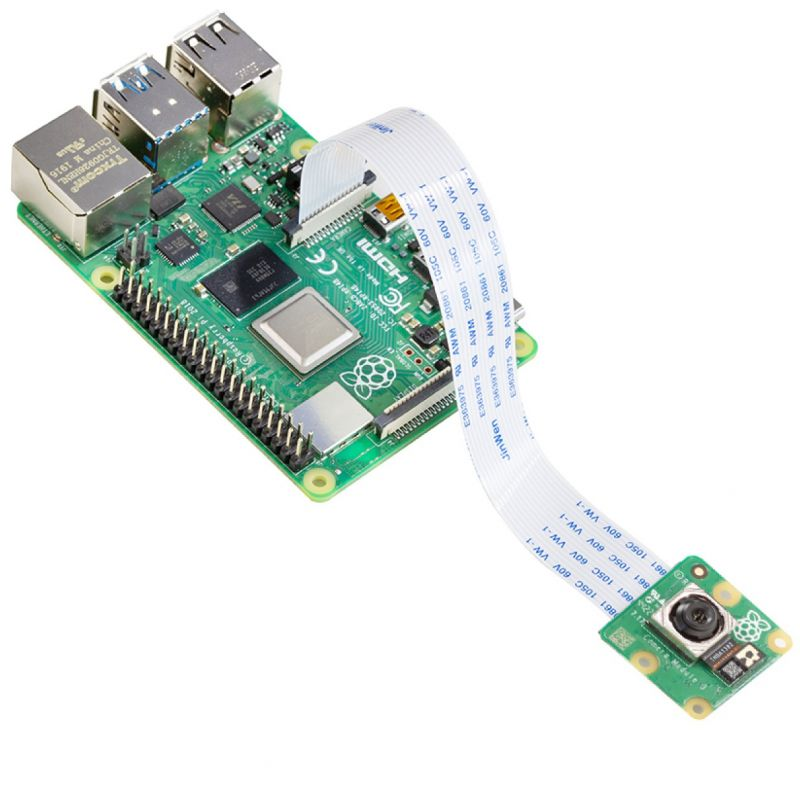
\includegraphics[width=0.3\textwidth]{images/Raspberry-Pi-Camera-Module-3-Wide.jpg}
    \caption{Raspberry Pi Camera Module~3 Wide mounted on a Raspberry Pi 5 board.}
    \label{fig:rpi_camera3_wide_board}
\end{figure}

The Camera Module~3 family is built around the \textbf{Sony IMX708} image sensor, which provides a resolution of approximately \textbf{11.9~MP} (4608$\times$2592 pixels).\cite{raspberrypi_camera_module_3_2026} In addition to its relatively high spatial resolution, the module supports \textbf{autofocus} through phase-detection autofocus and includes \textbf{HDR} capabilities, making it suitable for embedded vision tasks in which scene conditions may vary over time.\cite{raspberrypi_camera_module_3_2026,raspberrypi_camera_documentation_2026}

The \textbf{Wide} variant was selected because it provides a \textbf{120$^\circ$ diagonal field of view}, which is particularly useful in industrial environments where the camera must cover a relatively broad working area from a short mounting distance.\cite{raspberrypi_camera_module_3_2026} In the present setup, this characteristic is important because the system must observe the table area in which baked loaves are manually removed from the trays, which is relatively large and located at a distance of approximately 1.5~m from the camera.

\begin{figure}[h]
    \centering
    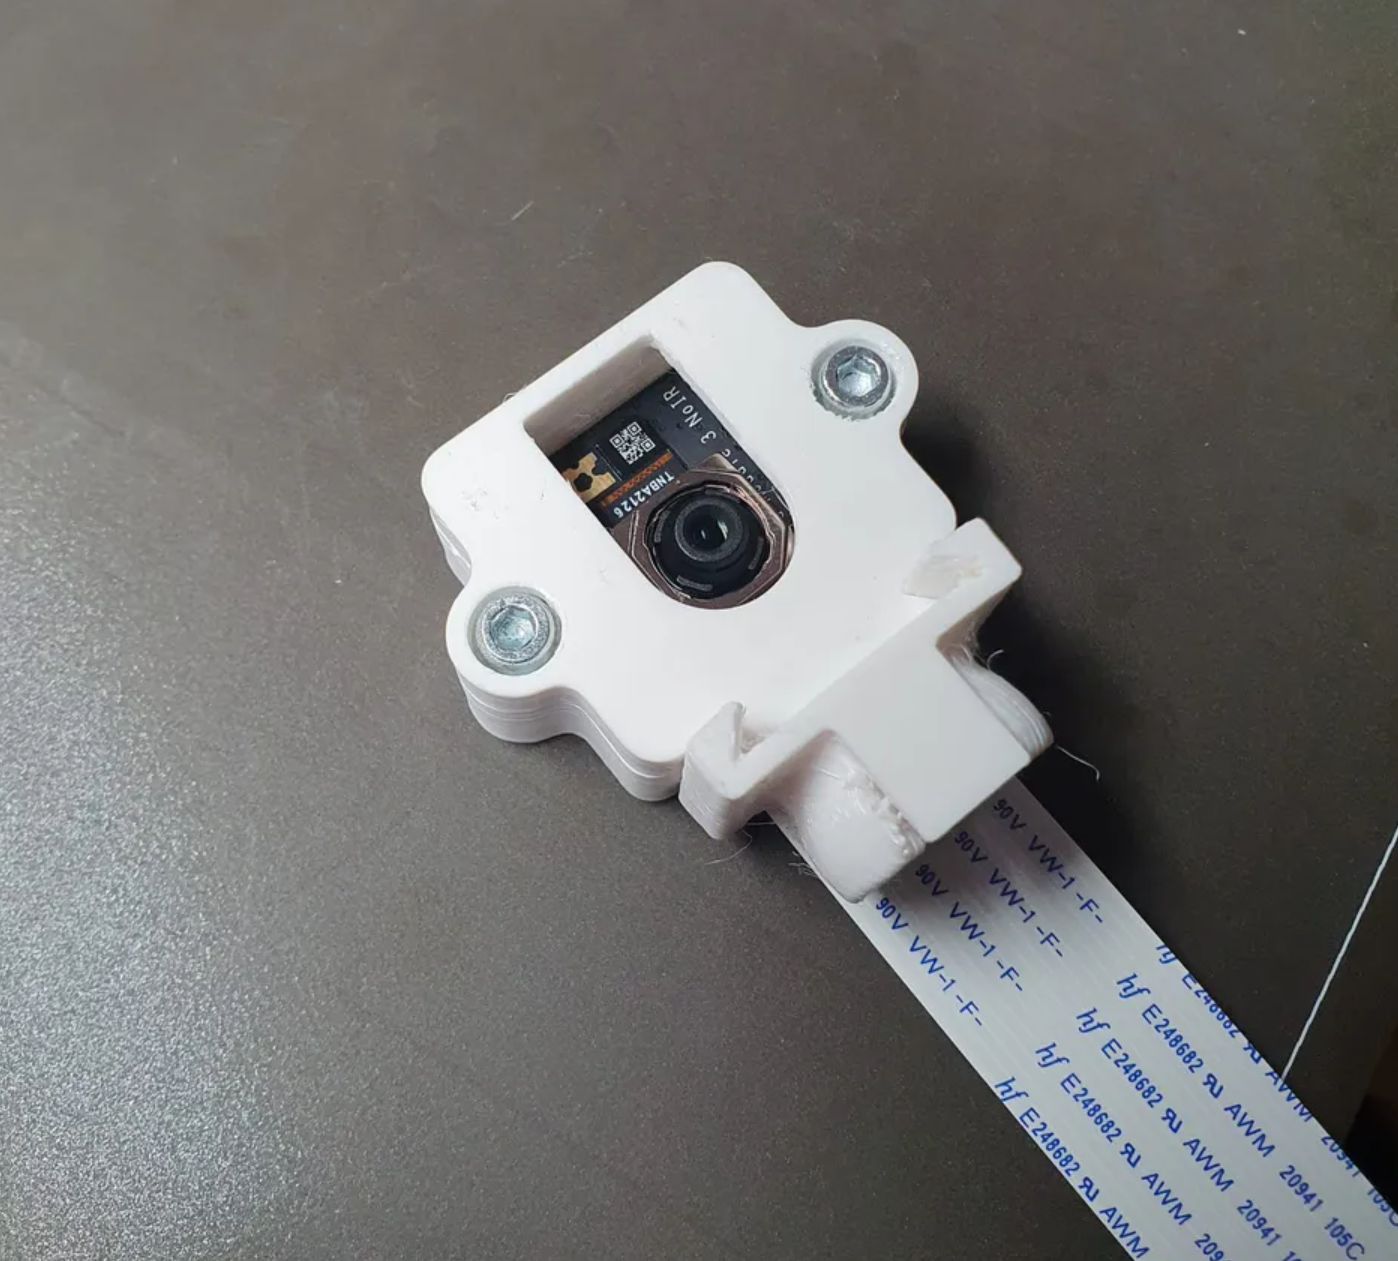
\includegraphics[width=0.4\textwidth]{images/Raspicam_3D-model.png}
    \caption{3D model of the Raspberry Pi Camera Module~3 Wide.}
    \label{fig:rpi_camera3_wide_model}
\end{figure}

To improve the practical integration of the camera into the Site~2 workstation, a dedicated housing solution was developed by starting from an existing online case model and modifying it for the specific constraints of the installation. The resulting enclosure was then fabricated through 3D printing. This solution was engineered to fit the geometry of the available station and to support a stable and repeatable mounting configuration for data acquisition. Besides providing mechanical protection, it improved cable management and helped maintain a more consistent camera placement under the specific operating conditions of the industrial environment, as shown in Figure~\ref{fig:rpi_camera3_wide_site2}.

\begin{figure}[h]
    \centering
    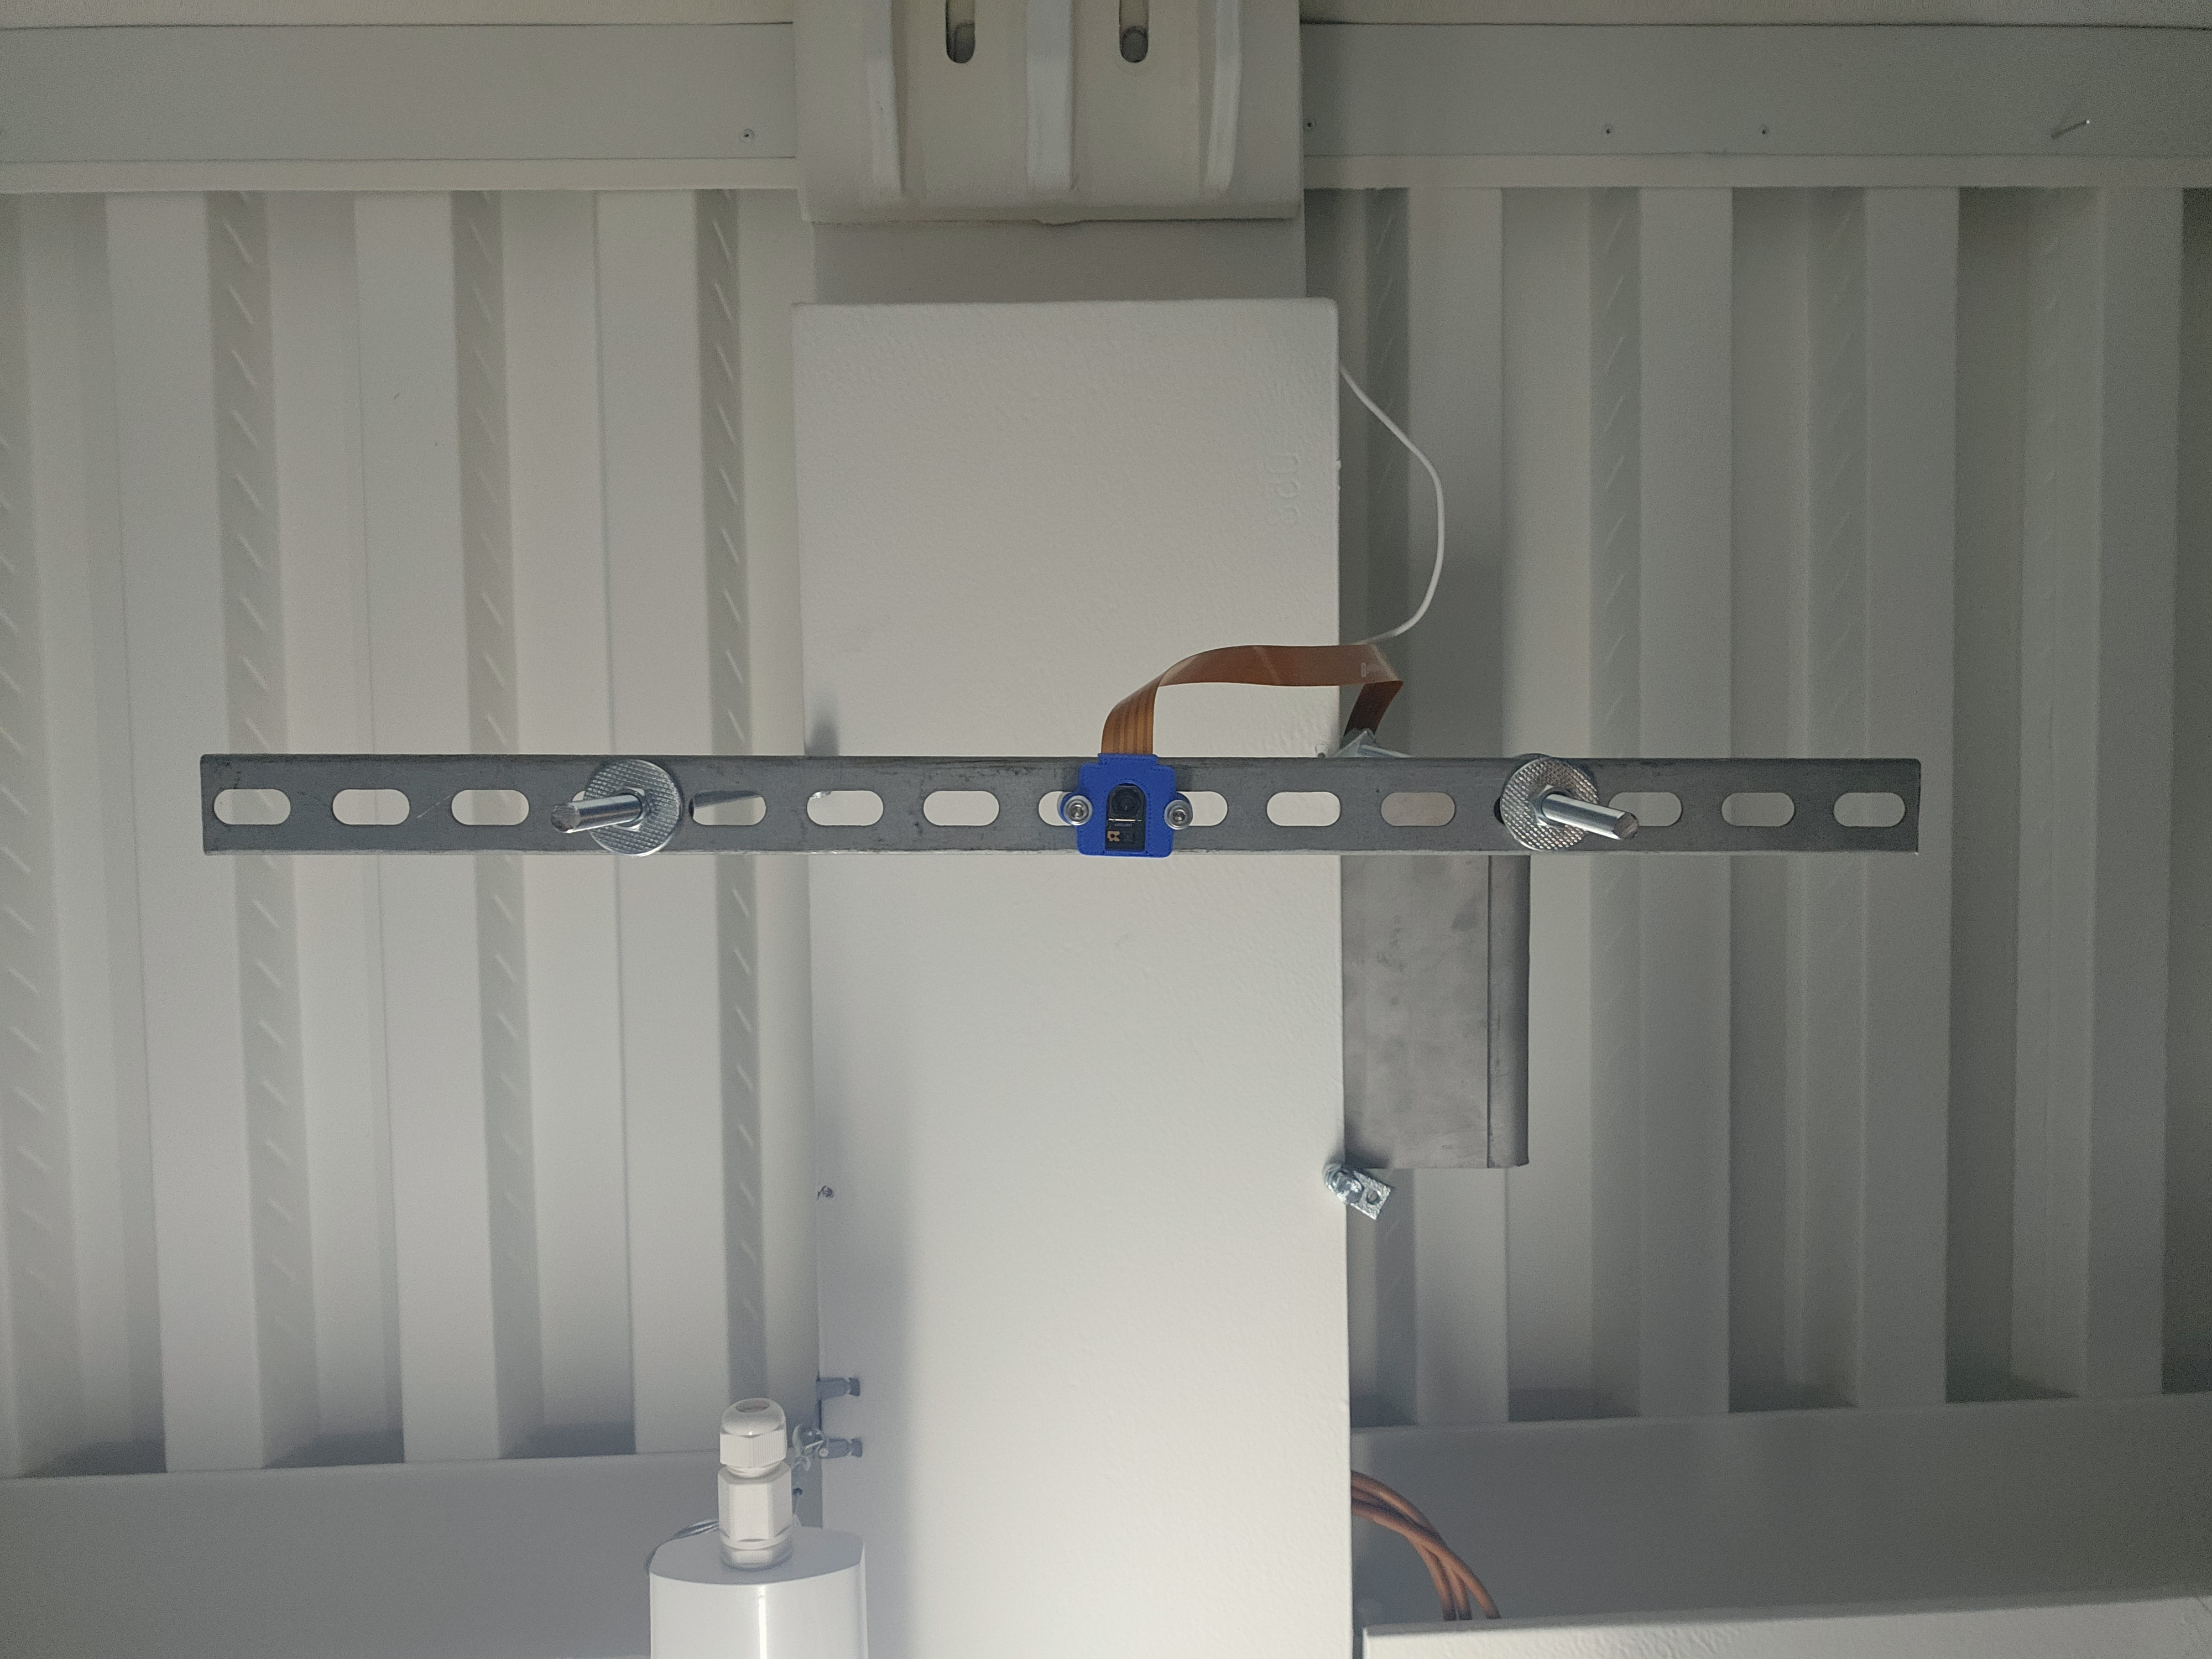
\includegraphics[width=0.5\textwidth, angle=90]{images/Raspberry_site2.jpg}
    \caption{Custom 3D-printed case for the Raspberry Pi Camera Module~3 Wide, placed in the Site~2 workstation.}
    \label{fig:rpi_camera3_wide_site2}
\end{figure}
\newpage
From an operational point of view, the camera module supports still-image acquisition at full sensor resolution and multiple video modes suitable for embedded computer-vision pipelines, including Full HD video and higher-frame-rate lower-resolution modes.\cite{raspberrypi_camera_module_3_2026,raspberrypi_camera_documentation_2026} The native integration with the Raspberry Pi ecosystem also simplifies software development through the official camera stack based on \textit{libcamera} and \textit{Picamera2}.\cite{raspberrypi_camera_documentation_2026}

For the purposes of this thesis, the Camera Module~3 Wide offers several practical advantages, including a field of view well suited to the inspection area, autofocus capability, and tight hardware and software integration with the Raspberry Pi 5. At the same time, the use of a monocular RGB camera also introduces some limitations. Unlike the Azure Kinect employed at Site~1, the Raspberry Pi Camera Module~3 Wide does not provide depth information and therefore cannot support direct 3D reconstruction. Moreover, because the sensing modality is purely RGB-based, the quality of the acquired data remains sensitive to lighting conditions, shadows, and viewpoint-dependent appearance changes. For this reason, illumination control and camera placement remain important aspects of the Site~2 setup, as illustrated in Figure~\ref{fig:faretto_sito2}. Overall, the Raspberry Pi Camera Module~3 Wide represents a suitable sensing solution for Site~2 thanks to its wide field of view, autofocus capability, compact form factor, and seamless compatibility with the Raspberry Pi platform.\cite{raspberrypi_camera_module_3_2026,raspberrypi_camera_documentation_2026}

\subsubsection{Picamera2 Library}
% !TeX root = ../../tesi.tex

For the integration of the Raspberry Pi Camera Module~3 Wide within the acquisition pipeline, the \textit{Picamera2} library was adopted.\cite{raspberrypi_picamera2_manual_2026,raspberrypi_picamera2_github_2026} Picamera2 is the Python interface built on top of the Raspberry Pi \textit{libcamera} stack and represents the modern replacement for the legacy Picamera interface.\cite{raspberrypi_picamera2_github_2026}

The library provides high-level access to camera initialization, stream configuration, frame acquisition, metadata handling, and camera controls such as exposure, gain, and autofocus.\cite{raspberrypi_picamera2_manual_2026} These features are particularly useful in embedded computer-vision applications, where the camera must be configured programmatically and integrated into a broader software pipeline.

In the present project, Picamera2 enabled direct access to RGB frames from Python, thereby simplifying the interaction between the camera and the processing software based on NumPy and OpenCV. This made it possible to implement image acquisition, parameter tuning, and frame extraction within the same software environment used for the rest of the pipeline.

Compared with lower-level camera handling, Picamera2 provides a practical abstraction that accelerates development while still exposing the controls needed for embedded deployment. This was particularly useful not only for the implementation of the acquisition pipeline itself, but also for the two-week automated data-collection phase, in which a stable and well-supported software interface was essential to manage continuous image acquisition and reliable data storage over extended periods. For this reason, Picamera2 represented a suitable software interface for Site~2, where ease of integration, reliability, and compatibility with the Raspberry Pi ecosystem were important design requirements.\cite{raspberrypi_picamera2_manual_2026,raspberrypi_picamera2_github_2026}

